\documentclass[twocolumn]{aastex62}

\newcommand{\vdag}{(v)^\dagger}
\newcommand\aastex{AAS\TeX}
\newcommand\latex{La\TeX}
\usepackage{amsmath}
\usepackage{physics}
\usepackage{hyperref}
\usepackage{natbib}
\usepackage[T1]{fontenc}
\usepackage[english]{babel}
\usepackage[utf8]{inputenc}
\usepackage{wasysym}

\begin{document}

\title{\Large AST5220-Milestone II: The Universes Opacity}

\author{Nils-Ole Stutzer}

\begin{abstract}
    
    \textit{The codes for this paper can be found at:} \newline \url{https://github.com/SagittariusA-Star/AST5220-Milestones}
\end{abstract}

\section{Introduction} \label{sec:Intro}
After having simulated the large scale background evolution of the universe in \cite{stutzer:2020}, we now want to compute the optical depth and the visibility function of the universe throughout its evolution. The computations made will expand upon the code previously made (\cite{stutzer:2020}). The optical depth and the visibility function are important quantities as, they essentially quantify how far a photon can travel in the universe before getting absorbed (when looking back in time). We make several assumptions, which amongst other things are that extinction through Thomson scattering provides the only extinction process and that the only baryons is hydrogen atoms. Also the epoch of reionization will be neglected, as a simplification. Computing the optical depth and visibility function is in principle not that hard, however, only if one is provided the density of free electrons. Thus, most of the work is finding the electron density evolution of the universe and from it the optical depth and visibility function. 

\section{Method} \label{sec:Method}
The formulas and equations presented here are provided by \cite{winther:2020}, unless otherwise stated.
\subsection{The Optical Depth}
As mentioned in the introduction computing the optical depth of the universe is in theory governed by fairly simple relations. When light travels through a medium, a given amount of photons are removed and added to the beam. The amount of photons that are added depend on the emissivity of the medium. We assume here that the gas the light travels through in the universe does have a negligible emissivity. Further more the amount of attenuation is given by the extinction coefficient
\begin{align}
    \alpha = n_e\sigma_T,
\end{align}
where we assume Thomson scattering on electrons to be the only mechanism to attenuate photons. Here $\sigma_T = \frac{8\pi}{3}\frac{\alpha^2\hbar^2}{m_e^2c^2}$
and $n_e$ are the Thomson cross section and the free electron density respectively. The optical depth is given by 
\begin{align}
    \tau(\eta) = \int_{\eta}^{\eta_0} n_e \sigma_T a d\eta',
\end{align}
where $a$ and $\eta$ are the scale factor and the conformal time of the universe.
We however will for practical reasons choose to solve for $\tau$ by solving the ordinary differential equation (ODE) 
\begin{align}
    \dv{\tau}{x} = -\frac{n_e\sigma_T}{H} = -\frac{n_e\sigma_T}{H}c, 
    \label{eq:tau_ode}
\end{align}
where $x = log(a)$ and $H = \frac{\dot{a}}{a}$ are the log-scale factor and the Hubble parameter respectively. The Hubble parameter is found by the Friedmann equation through the previously developed code in \cite{stutzer:2020}. We choose this ansatz instead of the integral, so we can use the \texttt{ODEsolver} routine provided by \cite{winther:2020}. We went from natural units to SI units in the last step. The equations provided by \cite{winther:2020} are given in natural units, however we want them to be in SI units, so as to enable solving in C++ using the constants in \texttt{Utils.h} provided by \cite{winther:2020}. We will show the dimensional analysis to go from natural units to SI on the example above, and than just provide the equations in SI units with all the constants from now on. As one can see in eq. (\ref{eq:tau_ode}) the l.h.s. of the equation if dimensionless because $\tau$ and $x$ both are. Thus the r.h.s. must be dimensionless too. We however see that the r.h.s. has units
\begin{align}
    1 = \frac{[n_e][\sigma_T]}{[H]}[c]^\alpha = \frac{\rm{m}^{-3}[\rm{m}^{2}]}{\rm{s}^{-1}}[c]^\alpha = \frac{\rm{s}}{\rm{m}}[c]^\alpha
\end{align}
The only physical constant that is reasonable to use here is thus the light speed $c$, with units $\rm{m}/\rm{s}$, thus $\alpha = 1$ in this case. Similarly, when having units for instance $\rm{Js}$ or $\rm{K}$ "too much" on one side in natural units, one can correct with the reduced Planck constant or Boltzmann constant to go to SI units. 

Now, as can be seen from eq. (\ref{eq:tau_ode}), there is one problem however; we need to know the electron density. We will address this problem in the next subsection.

\subsection{The Free Electron Fraction and Density}
In order to compute the optical depth we need to know the free electron density $n_e$. We can compute this through the free electron fraction $X_e$ and use the baryon, i.e. hydrogen density as a translational factor. We thus get that the electron density as a function of the electron fraction and the hydrogen (baryon) density is 
\begin{align}
    n_e = X_e n_H,
\end{align}
where 
\begin{align}
    n_H = n_b \approx \frac{\rho_b}{m_H} = \frac{\Omega_{b0} \rho_{c0}}{m_H a^3},
\end{align}
where we have assumed all baryons to be in hydrogen. This should be a reasonable approximation since the hydrogen atoms comprise almost all of the baryons in the universe. Here the baryon density parameter and the critcal density today are given as their regular expressions found in and computed in \cite{stutzer:2020}. The time dependence of the baryon density is solely in the scale factor dependent $a^{-3} = e^{-3x}$ factor. 

The remaining job to find $n_e$ is to find the electron fraction $X_e$. This turns out to be the hardest part of the total work. We can find $X_e$ through solving the Boltzmann equation for a recombination/ionization reaction of the type $e^{-} + p^{+} \rightleftharpoons H + \gamma$. At early times the energies of the constituent particles were high enough to keep this reaction in equilibrium. As long at the reaction is close to equilibrium Saha's approximation \citep[p. 70]{dodelson:2003} ensures that 
\begin{align}
    \frac{n_e n_p}{n_H} = \frac{n_e^{(0)}n_p^{(0)}}{n_H^{(0)}},
\end{align}
where the $n_i^{(0)}$ denote the equilibrium distribution species $i$. As the universe's charge is net zero, we can safely assume their to be as many free electrons as protons, i.e. $n_e = n_p$. Using this assumption we get the Saha equation for recombination given as 
\begin{align}
    \frac{X_e^2}{1 - X_e} = \frac{1}{n_b} \left(\frac{m_e
    T_bk_B}{2\pi\hbar^2}\right)^{3/2} e^{-\epsilon_0/T_bk_B} \equiv R.
    \label{eq:Saha_eq}
\end{align}
Here $m_e$ and $\epsilon_0$ are the electron mass and the ionization energy of hydrogen respectively \citep[]{winther:2020}. The temperature $T_b$ is the baryon temperature, which in principle should be found separately, however we can approximate it to the radiation temperature $T_r$ \citep[]{winther:2020}. It is is thus given as $T_b =
T_r = T_{\rm CMB} / a = 2.7255 \textrm{K} / a$.

Because eq. (\ref{eq:Saha_eq}) is a simple quadratic equation its solution is simply 
$X_e = \frac{1}{2} (-R \pm \sqrt{R^2 + 4R})$, where $R$ stand for the r.h.s. of Saha's equation. Note that only the "+"-solution is physically valid. We will also briefly come back to this solution in sec. \ref{subsec:implementation} to discuss some numerical issues with this solution.

We have, however, not yet found a complete solution, since the Saha equation is only valid if $X_e$ is close to unity. To solve for $X_e$ if $X_e$ falls below some tolerance, which we choose to be $X_e = 0.99$ than we need to use the better approximation to $X_e$ given by the Peebles' equation
\begin{align}
    \frac{dX_e}{dx} = \frac{C_r(T_b)}{H} \left[\beta(T_b)(1-X_e) - n_H
              \alpha^{(2)}(T_b)X_e^2\right].
    \label{eq:peebles}
\end{align}
Here 
\begin{align}
    C_r(T_b) &= \frac{\Lambda_{2s\rightarrow1s} +
              \Lambda_{\alpha}}{\Lambda_{2s\rightarrow1s} + \Lambda_{\alpha} +
              \beta^{(2)}(T_b)}, \\
    \Lambda_{2s\rightarrow1s} &= 8.227 \textrm{s}^{-1}\\
    \Lambda_{\alpha} &= H\frac{(3\epsilon_0)^3}{(8\pi)^2 (\hbar c)^3 n_{1s}}\\
    n_{1s} &= (1-X_e)n_H \\
    \beta^{(2)}(T_b) &= \beta(T_b) e^{3\epsilon_0/4T_bk_B} \\
    \beta(T_b) &= \alpha^{(2)}(T_b) \left(\frac{m_e
              T_bk_B}{2\pi \hbar^2}\right)^{3/2} e^{-\epsilon_0/T_bk_B} \\
    \alpha^{(2)}(T_b) &= \frac{8}{\sqrt{3\pi}}
              \sigma_T c\sqrt{\frac{\epsilon_0}{T_bk_B}}\phi_2(T_b) \\
    \phi_2(T_b) &= 0.448\ln(\epsilon_0/T_bk_B),
\end{align}
are constants describing simple atomic transitions between the ground state of hydrogen (1s) and the second exited state (2s) \citep[]{winther:2020}. Importantly, Peebles equation is also simply a first order approximation for $X_e$. A more thorough handling would be to include different atomic species as well as several more transitions. We will however stick with our two level hydrogen model. Note we have included all the necessary constants to translate the system of equation to the SI system. 

The Peebles' equation is simply another linear ODE which we can simply solve using the \texttt{ODEsolver}-routine by \cite{winther:2020} as discussed in sec. \ref{subsec:implementation}. Now that we have an expression for $X_e$ we can as mentioned earlier easily find $n_e$ and again use the \texttt{ODEsolver}-routine to find the optical depth $tau$.

The only remaining quantity we need to compute is the visibility function 
\begin{align}
    \tilde{g}(x) = -\dv{\tau}{x} e^{-\tau},
\end{align}
which quantities the probability density for a photon to scatter at a given log-scale factor $x$. It is a true probability density function (PDF), meaning it  integrates to unity over all of the universes history. 

\subsection{Implementation}\label{subsec:implementation}
As mentioned previously the main goal of this paper is to compute $X_e$ to find $tau(x)$ and $\tilde{g}(x)$. The main strategy is to loop through values of $x$ and at each step compute the solution of Saha's equation. If this solution is at some point below the tolerance $X_e = 0.99$ we switch to Peebles' equation. When in the Peebles regime we set up an ODE with one step for each (outer) loop iteration over $x$. The initial condition for each iteration is the value of $X_e$ in the previous iteration. The ODE is than for each iteration stepped forward from the previous to the current value of $X_e$, which is subsequently added to an array. Alternatively one could have solved all of the Peebles regime in one go, than exit the $x$ loop. However, we found the step wise method to be more intuitive. The solving of the ODE was done with the \texttt{ODEsolver}-routine by \cite{winther:2020}.

In the same loop over $x$ we simultaneously compute $n_e$ as a function of $x$. The resulting solutions for $X_e$ and $n_e$ were than splined using the \texttt{Spline}-routine by \cite{winther:2020}, in order to get a more continuos callable representation of the two quantities. Since both $X_e$ and $n_e$ vary a lot through the universes history, we made a spline of the logarithm of the quantities instead of the quantities themselves to prevent numerical errors.

Importantly there were two numerical subtleties when solving the Saha and Peebles equations. The first was that when solving the quadratic Saha equation, the case when the r.h.s. $R$ of eq. (\ref{eq:Saha_eq}) can result in something of the form $-R + R\sqrt{1 + 4/R} = -R + R = 0$, i.e. $\text{"large" - "large"} = 0$, because a computer lets $1 + \text{"small"} = 1$. Then $X_e = 0$ even though it should be $X_e = 1$. This happens when $R$ becomes large, i.e. at early times. To solve the problem we consider the solution 
\begin{align}
    X_e &= \frac{1}{2} (-R + \sqrt{R^2 + 4R}) = \frac{1}{2} (-R + R\sqrt{1 + 4/R})\\
        &\approx \frac{1}{2} (-R + R(1 + 2/R)) = 1,
\end{align}
using a taylor expansion to first order, since $4/R \ll 1$ when $R\gg 1$. This yields the correct result $X_e = 1$ at early times. We thus simply include an \texttt{if}-test to check for this, in which case $X_e = 1$ and else we compute the solution according to the regular formula. We chose to use $4/R = 10^{-9}$ as the tolerance, under which we set $X_e = 1$. 

The second subtlety is that in the Peebles equation we have expressions containing exponential functions with positive exponents that can be very large at late times. In particular we have $\exp\left(3\epsilon_0 / 4T_b k_B\right)$ in the expression for $\beta^{(0)}$ which can easily overflow. Fortunalty, there is a relatively easy solution; simply combine the expressions for $\beta^{(0)}$ and $\beta$ directly. This way the exponential factor in $\beta^{(0)}$ becomes $\exp\left(-\epsilon_0 / 4T_b k_B\right)$, which in case of a large fraction $\epsilon_0 / T_b k_B$ will simply underflow and give zero, which is alright in our case.

Now, having solved for the free electron density, finding $\tau$ and subsequently $\tilde{g}$ is easy. We simply set up an ODE for $\tau$ and solve it using the \texttt{ODEsolver}-routine \citep[]{winther:2020}, all in one go. There is, however, one thing we have to handle. Since the \texttt{ODEsolver}-routine cannot solve the ODE backwards with initial condition $\tau(x = 0) = 0$, and $\tau$ at early times is unknown. There is, however, a simple trick; simply use some random initial condition, and find $\tau(x=0)$ (in our case always the last array value of the solution with random initial condition for $\tau$), then subtract $\tau(x = 0)$ from all $\tau(x)$ values. This way we simply move the origin to correct for the wrong initial condition. 

The values for $\tau(x)$ are than splined using the \texttt{Spline}-routine \citep[]{winther:2020}. We found that extracting the first and second derivative of $\tau$ from its spline, resulted in some numerical noise oscillations close to the present age. We thus used the analytical expression for $\dv{\tau}{x}$ to make a spline of it directly, and than extract the second derivative of $\tau$ from the spline of the first derivative instead. This largely resolved the problem. 

Computing the visibility function $\tilde{g}(x)$ is now just a matter of using the computed splines for $\tau$ and $\dv{\tau}{x}$. A spline is than also made for the visibility function, and the first and second derivatives are found through the spline. 

Finally the results are printed to a data file and subsequently plots are produced using a Python script.


\section{Results/Discussion}\label{sec:Results}

\begin{figure*}
    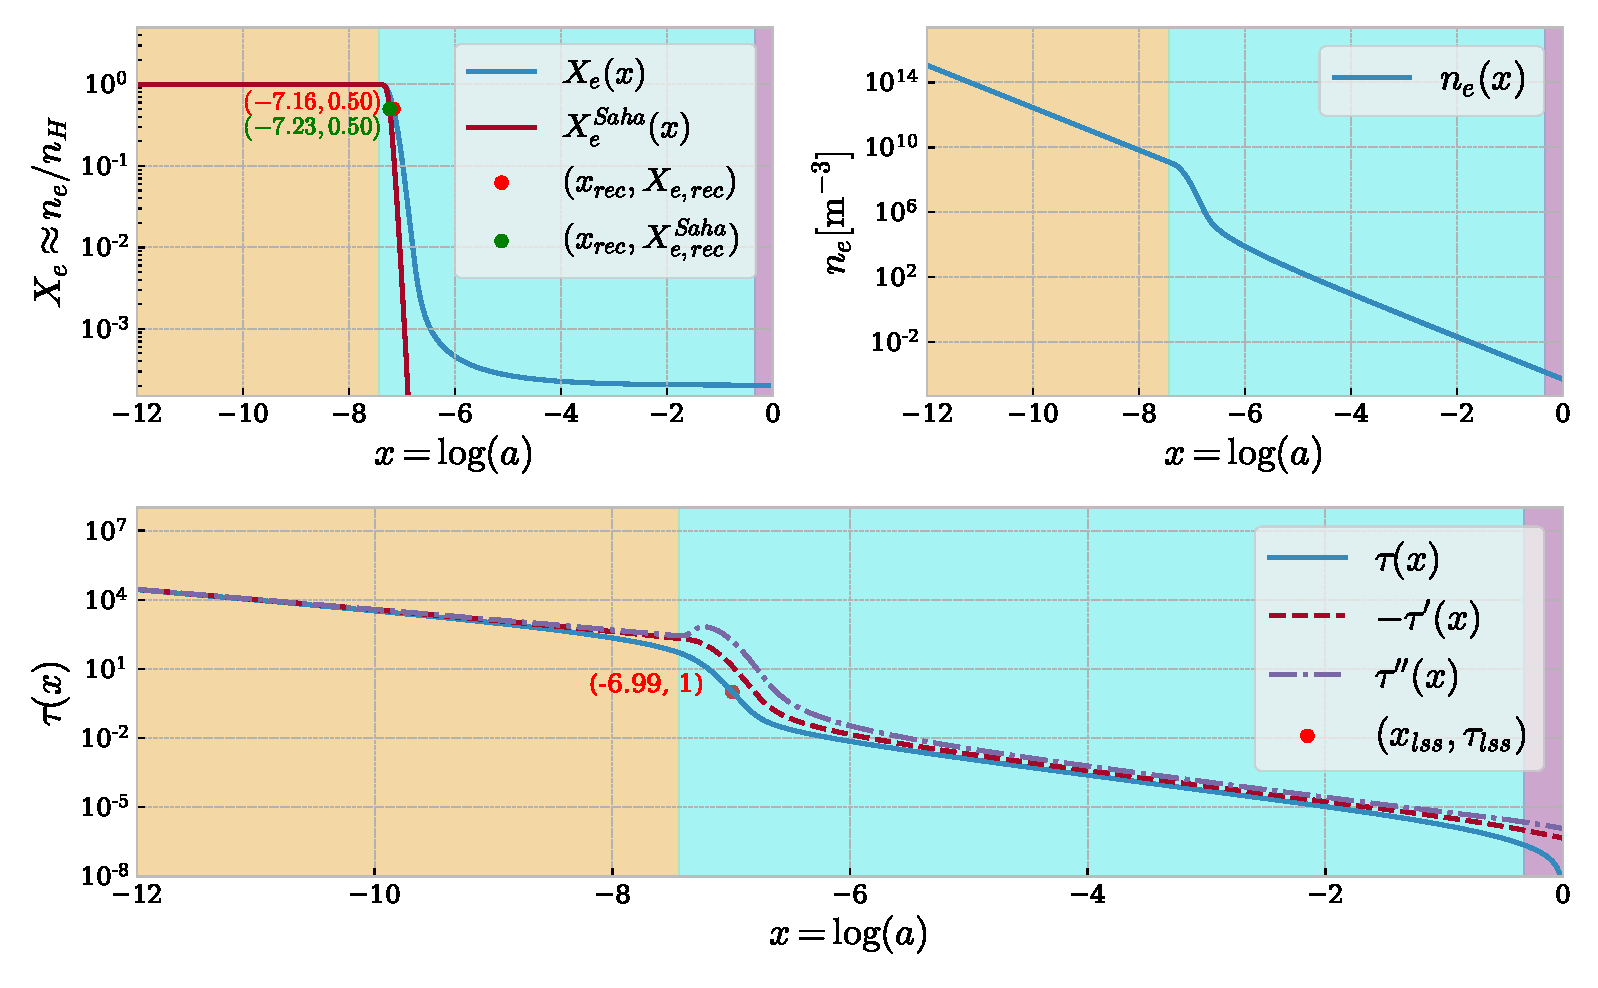
\includegraphics[scale = 0.65]{Figures/Xe_ne_tau.pdf}
    \caption{\textbf{Upper left}: Figure showing the free electron fraction $X_e$ 
    as a function of the log-scale factor $x$. \textbf{Upper right}: Figure showing the free electron density $n_e$
    as a function of the log-scale factor $x$. \textbf{Lower panel}: Figure showing the optical depth $\tau(x)$ of the universe due to 
    Thomson scattering on free electrons only, as well at the derivative $\tau'(x)$ and second oder derivative $\tau''(x)$ w.r.t 
    and as functions of the log-scale factor $x$. \textbf{Note}: The background color in all the plots shows the epoch of dominance
    for reference. Yellow markes the era of radiation dominance, blue the epoch of matter domination
    and purple corresponds to the epoch of dark energy. The color domain is found by checking 
    when the corresponding density parameter is dominant,
    however, in reality the transitions between each epoch should be smoother than shown.}
    \label{fig:Xe}
\end{figure*}

\begin{figure*}
    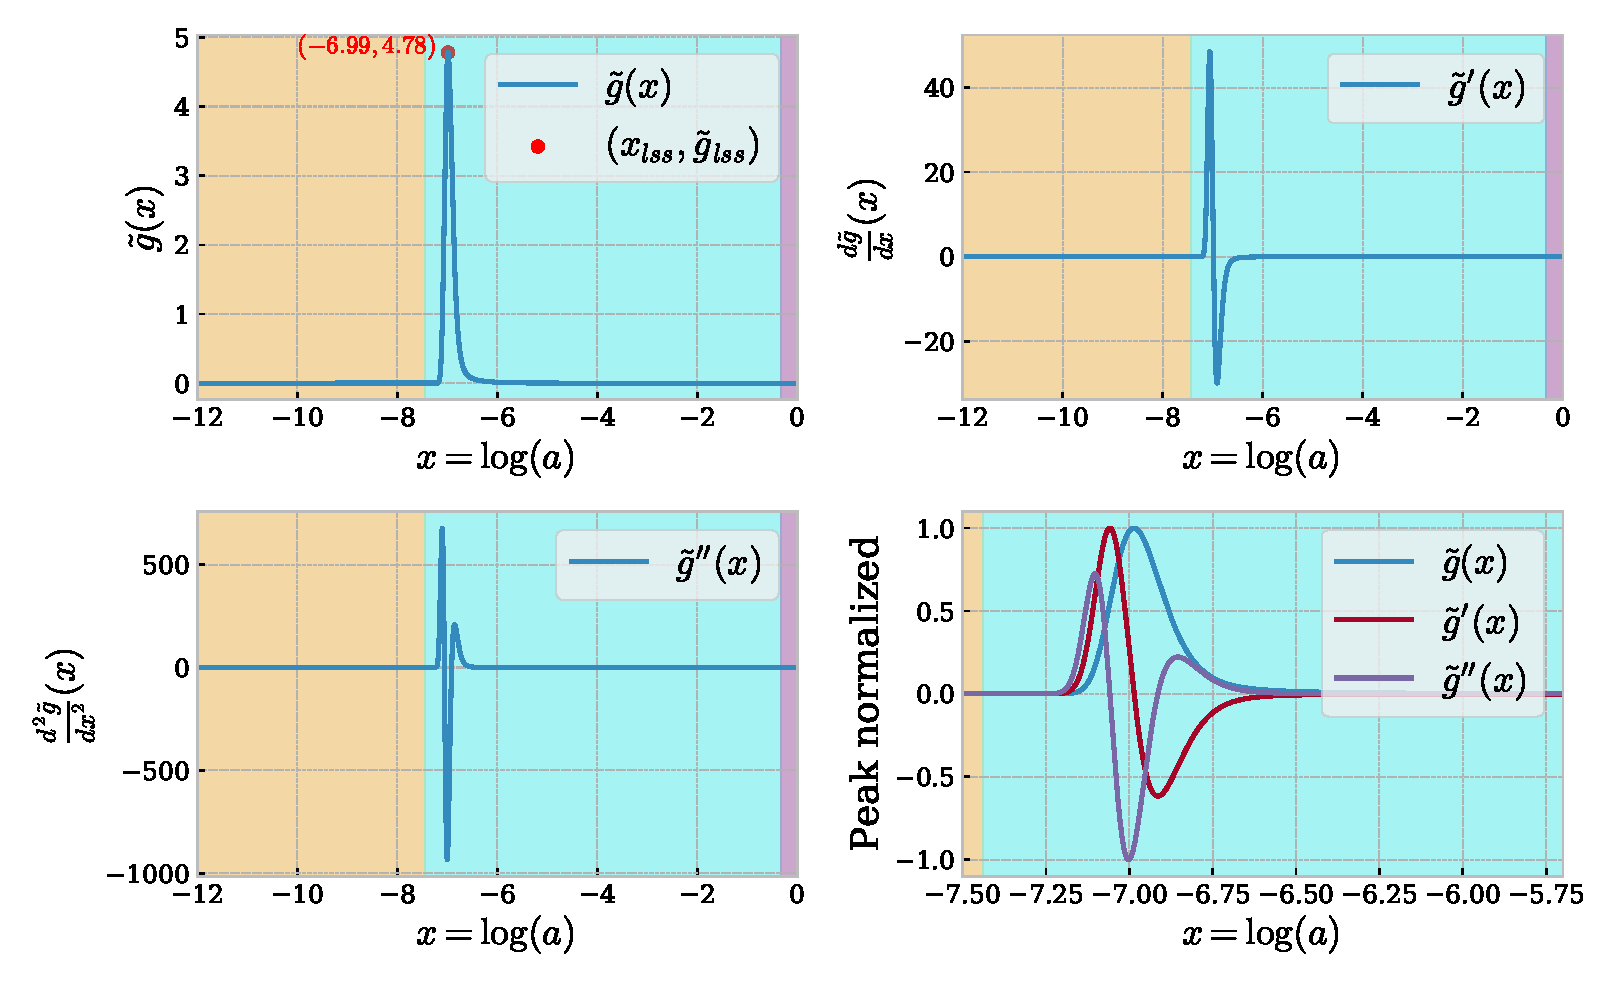
\includegraphics[scale = 0.65]{Figures/g_tilde.pdf}
    \caption{\textbf{Upper left}: Figure showing the un-normalized visibility function $\tilde{g}$ as a function of the log-scale factor $x$.
    The red dot markes the peak of $\tilde{g}$ 
    and its $x$ value corresponds to the log scale factor of the surface of last scattering. 
    \textbf{Upper right}: Figure showing the un-normalized first order derivative of $\tilde{g}$ w.r.t. and as a function of the log-scale factor. 
    \textbf{Lower left}: Figure showing the un-normalized second order derivative of $\tilde{g}$ w.r.t. and as a function of the log-scale factor.
    \textbf{Lower Right}: Figure showing the visibility function and its first two derivative together in one plot, where all functions are normalized to their respective extremum value (peak or valley). Also we have zoomed in somewhat to show more details.
    }
    \label{fig:g_tilde}
\end{figure*}

\section{Conclusion} \label{sec:Conclusion}


\bibliography{ref}
\bibliographystyle{aasjournal}
\end{document}